\clearpage
\section{Image reduction}
Calibration frames and science frames have been already taken. Dark frames are not provided and not necessary, since dark currents can be neglected in this case due to proper cooling. Here these images will get inspected and reduced as explained before.
\subsection{Raw-image inspection}
Calibration images are firstly visually inspected using \verb|ds9| with \verb|zscale| setting. Figure~\ref{fig:bias} and~\ref{fig:flat} are examples of bias and flat frames. Note that images shown here are not the whole images.
\begin{figure}[H]
   \centering
   \begin{subfigure}[b]{0.5\textwidth}
   \begin{center}
   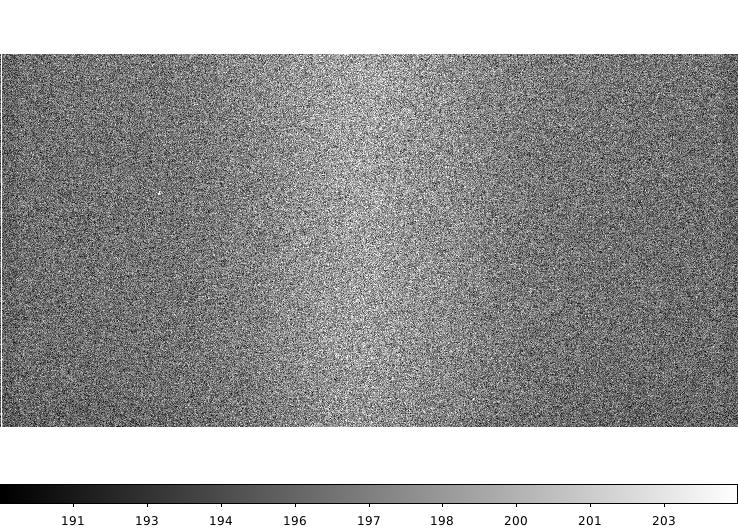
\includegraphics[width=0.8\linewidth]{bias.jpeg}
   \end{center}
   \caption{Bias frame}
   \label{fig:bias}
   \end{subfigure}%
   \begin{subfigure}[b]{0.5\textwidth}
   \begin{center}
   \includegraphics[width=0.8\linewidth]{flat.jpeg}
   \end{center}
	\caption{Flat frame. Color legend was unfortunately not included in screenshot.}
   \label{fig:flat}
   \end{subfigure}
	\caption[Calibration frames. Shown images are only central part of whole images.]{Calibration frames. Shown images are only central part of whole images.\footnotemark}%
\end{figure}
\footnotetext{Unfortunately some images were taken without the color/gray scale.}

Average bias level is somewhat near $200$. This values changes, though not so obvious in figure~\ref{fig:bias}, throughout the image. Left and right sides are significantly darker, meaning less bias. Presumably it is related to geometry and layout of CCD chip. Sometimes one can see quite large white dots in bias picture. Positions of these white dots vary from image to image. Because of its significant size comparing to other noises, they are mostly likely to be cosmic rays, as hinted by~\cite{manual}.

Middle of bias frame is chosen to calculated background and sigma, due to its lack of large-scale variation. Output of \verb|imstats| gives us mean and sigma: $\num{198.72 +- 2.59}$. Noise here should be readout variations and random fluctuations~\cite{manual}.

In flat-field, most obvious feature is black circles or doughnuts. These are dusts on dewar windows and/or filter~\cite{manual}. This results in lower photon counts, thus black in flat-field images. They are not on CCD chips, since they are not properly focused. Some large-scale structure can be seen. It can be explained by different quantum efficiency at different area of CCD. There are quite a lot small sharp black dots visibly. They are most likely to be bad pixels and dust directly on CCD chip.

Each flat-field has different exposure time. One can try to find correlation between mean value of image and exposure time using commands provided in~\cite{manual}. Ratios between these two goes down with increasing exposure time. Firstly of all, CCD chips should be saturated here, since with exposure time, mean values goes down. One possibility is that read-out noise in circuit gets averaged out with long exposure time, thus lower ratio.
\begin{figure}[H]
   \centering
   \includegraphics[width=0.6\linewidth]{mean_exp.pdf}
   \caption{Mean values (red) with sigmas and the ratios (blue) against exposure time of flat-field images.}%
\end{figure}

In science frame one can clearly see doughnut structures and sharp black dots as in flat-field frames. Between exposure, most out-standing change would be that telescope is moving around. 
\begin{figure}[H]
   \centering
   \includegraphics[width=0.8\linewidth]{science.jpeg}
   \caption{An example of science frame.}%
   \label{fig:science}
\end{figure}

We use \verb|image008068.fits| as an example and compute mean and sigma in area without bright objects. Values are \num{693.20 +- 19.00}. It is greater than the mean value of bias frame. This is easy to understand, since science frame must contain sky. 

\subsection{Image reduction}
Several science frames containing source \verb|SDSS1650+4251|  are taken from one filter ($R$). Now these images with be reduced with help of calibrations frames and some more in \verb|theli|. \verb|theli| mainly consists of several tabs or processing groups. Each of following paragraph corresponds one processing group/

\paragraph{Initialise}  First off, \verb|theli| should be properly reset and initialised. Number of CPU cores and instrument (telescope) are specified accordingly. Paths containing bias, flat, and science frames are filled in.

\paragraph{Preparation}
Through this processing group, headers contained in \verb|.fits| files can be split and/or corrected. Comparison of headers before and after corrections reveals
\begin{itemize}
   \item size in $x$ and $y$ are swapped, meaning orientation of images has been changed,
   \item (useless) information, e.g.~comments, CCD info, Date, and etc., has been removed,
   \item lots of lines starting with \verb|DUMMY| have been added.
\end{itemize}
They are more changes, but the listed alterations are most noticeable.

\paragraph{Calibration}
In this step, calibration frames are getting co-added. In co-addition process, images are stacked on top of each other, while making sure each object falls onto the same pixel~\cite{manual}. By doing this and in the end only calibrating with co-added images, random noises will get averaged out.  

After co-addition, bias frames are free of small white dots as seen before and flat frames get a bit brighter. One can further computer noise dispersion of co-added bias frame and single bias frame. They are respectively \num{0.72} and \num{2.27}. So noise level in co-added images is much lower.

The minimal value in normalised flat-field is $0$. Dithering during co-addition helps to remove bright objects (stars and etc.).

\paragraph{Background modelling}
In this processing group, only background model correction is selected, where a superflat and fringe model is created and applied. Its configurations are set according to~\cite{manual}: $\verb|DT| = 1.0$, $\verb|DMIN|=10$, mask expansion factor$=3$, \verb|median| combination, \verb|divide smoothed model, subtract fringes| method, smoothing kernel for background model $=256$.

In superflat, one can clearly see fringes pattern. Fringes and background sky can be extracted with smoothing process. In \verb|SDSS1650+4251_R_block0_1_fringe.fits|, there is only fringes visible and in \verb|SSD1650+4251_R_block0_1_illum.fits| only smooth gradient, i.e.~background.

Correction given by illumination is roughly \num{500} (counts). Fringes are removed after correction, see figure~\ref{fig:before} and~\ref{fig:after}.
\begin{figure}[H]
   \centering
   \begin{subfigure}[t]{0.7\textwidth}
   \begin{center}
   \includegraphics[width=\linewidth]{before.jpeg}
   \end{center}
   \caption{Before correction. Pay attention to top left corner.}
   \label{fig:before}
   \end{subfigure}
   \begin{subfigure}[t]{0.7\textwidth}
   \begin{center}
   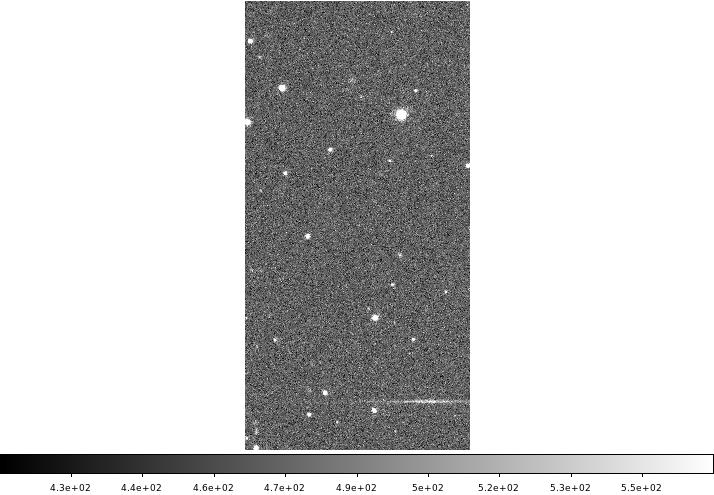
\includegraphics[width=\linewidth]{after.jpeg}
   \end{center}
   \caption{After correction. Pay attention to top left corner.}
   \label{fig:after}
   \end{subfigure}
	\caption{Background modelling}
\end{figure}

\paragraph{Weighting} 
In this step, weighting and masking are performed to compensate bad pixels and different quantum efficiency. Global weights and WEIGHTS are created and applied.

\paragraph{Astrometry/Photometry}
This processing group matches dithered frame to standard astrometric coordinates and performs photometry calibration. Astrometric reference catalog is retrieved using setting provided in~\cite{manual}: \verb|Web(france)|, \verb|SDSS-DR9|, \verb|mag limit|9|, \verb|radius=5'|. $421$ objects are found. Then detection threshold is set to $2\sigma$ and minimal area for detection of $10$ pixels.

Matching is done with \verb|Scamp| with \verb|DISTORT_DEGREES=1|. Calculation is done after \verb|Scamp| has been correctly configured. After this, numerous check plots are generated.

\paragraph{Co-addition} 
Frames are astrometrically co-added, subtracted by sky/background, and normalised to exposure time of \SI{1}{\second}.  Settings are again provided in~\cite{manual}: \verb|Model the sky|, \verb|DT=1|, \verb|DMIN=10|, \verb|kernel width=256|, outlier rejection to $4$. After co-addition, newly generated frames can be found in new folder with name starting with \verb|coadd_|, see figure~\ref{fig:coadds}. Logically, they have the same shapes and brightest region of co-added weight frame also has high S/N ratio. Indeed, one can compute noise using \verb|imstats| as before. RMS of region free off bright objects is \num{0.02}, far lower than previous single frames. This can be properly understood, since frames are co-added and then normalised, resulting high S/N ratio.
\begin{figure}[h]
   \centering
   \begin{subfigure}[t]{0.8\textwidth}
   \begin{center}
   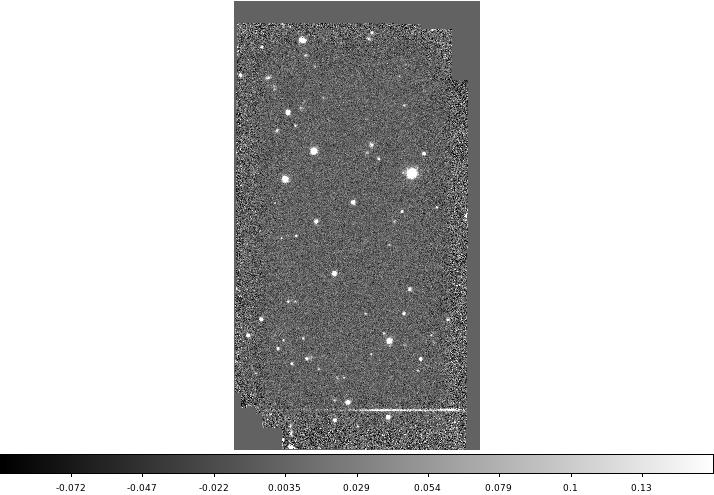
\includegraphics[width=1\linewidth]{coadd.jpeg}
   \end{center}
   \caption{Co-added frame}
   \label{fig:coadd}
   \end{subfigure}
   \begin{subfigure}[t]{0.8\textwidth}
   \begin{center}
   \includegraphics[width=1\linewidth]{coadd.weight.jpeg}
   \end{center}
   \caption{Co-added weight}
   \label{fig:coadd-weight}
   \end{subfigure}
   \caption{Frames generated after co-addition}%
   \label{fig:coadds}
\end{figure}

\clearpage
\section{PSF extraction}
In this section, point-spread-function (PSF) will be extracted. First of all, the target need to be found using standard coordinates: $\text{RA} = 16^\text{h}50^\text{m}43.4^\text{s}$, $\text{DEC}=+42\degree 51'49''.00$. In \verb|ds9|, coordinates can be turned on with \verb|coordinate grid| option, see figure~\ref{fig:coor-grid}. As mentioned in~\cite{manual}, this target consists of two lensing images, but the separation have similar size as a typical seeing, so images are blended.
\begin{figure}[ht]
   \centering
   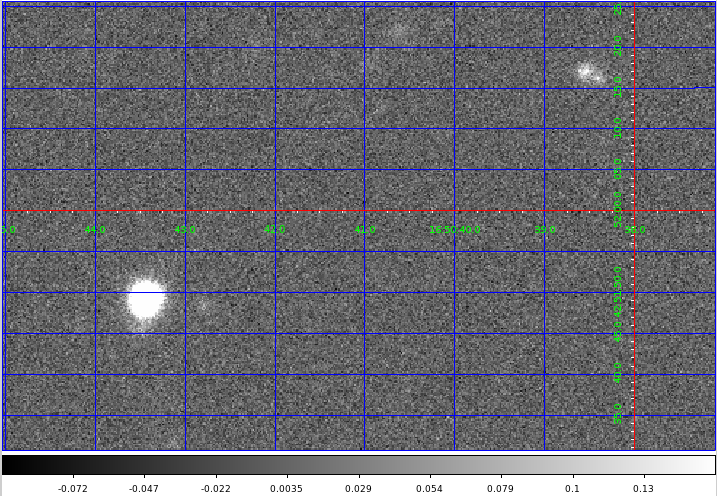
\includegraphics[width=0.6\linewidth]{coor.png}
   \caption{Co-added frame with coordinate grid. Target is the left-bottom bright object.}%
   \label{fig:coor-grid}
\end{figure}

In order to perform component fitting, PSFs of other various objects need to be extracted. One can gain more detailed information about objects using \verb|iraf| task \verb|imexam|. 

\begin{figure}[ht]
   \centering
   \begin{subfigure}[t]{0.5\textwidth}
   \begin{center}
   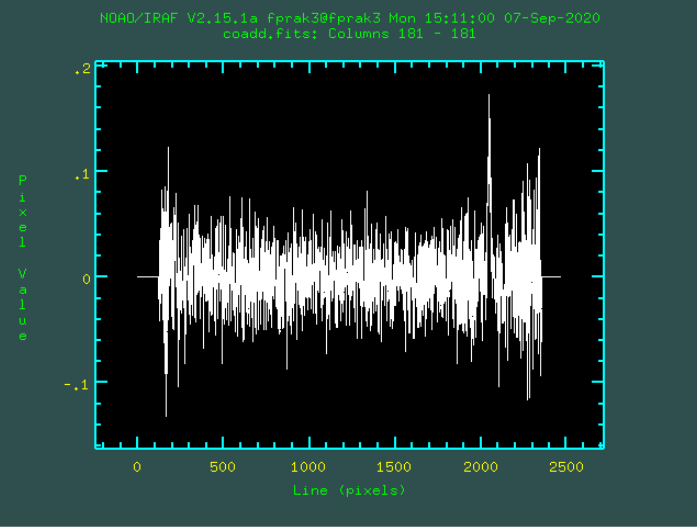
\includegraphics[width=0.9\linewidth]{galaxyColumn.png}
   \end{center}
   \caption{Column plot}
   \end{subfigure}%
   \begin{subfigure}[t]{0.5\textwidth}
   \begin{center}
   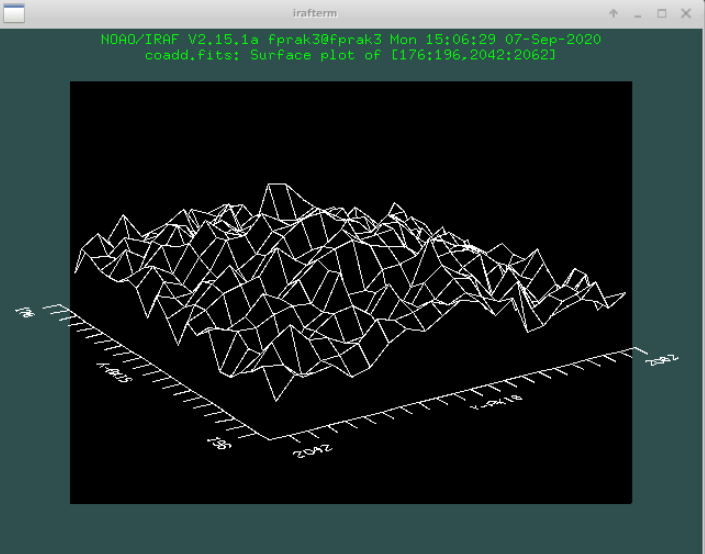
\includegraphics[width=0.9\linewidth]{galaxySurface.png}
   \end{center}
   \caption{Surface plot}
   \end{subfigure}
   \caption{Example plots of a galaxy}%
   \label{fig:galaxyPlots}
\end{figure}

There are mainly two categories of objects: stars and galaxies. Since galaxies contain a number of radiation sources, their full widths at half maximum (FWHMs) are typically larger than single stars. Indeed, that is what we see. FWHMs of stars are $\sim\num{6+-1}$ pixels, of galaxies $\sim\num{9+-1}$ pixels. Identification of stars and galaxies can be easier with various plots provided by \verb|imexam|. Two example plots each are figure~\ref{fig:galaxyPlots} and~\ref{fig:starPlots}. In contour plots, stars appear to be (almost perfect) concentric circles while galaxies are messier. Radial profiles of star have clear trend while they are scattered for galaxies. These plots support previous argument regarding differentiation stars from galaxies.
\textcolor{blue}{seeing in arcseconds?}
\begin{figure}[ht]
   \centering
   \begin{subfigure}[t]{0.5\textwidth}
   \begin{center}
   \includegraphics[width=0.9\linewidth]{starCoumn.png}
   \end{center}
   \caption{Column plot}
   \end{subfigure}%
   \begin{subfigure}[t]{0.5\textwidth}
   \begin{center}
   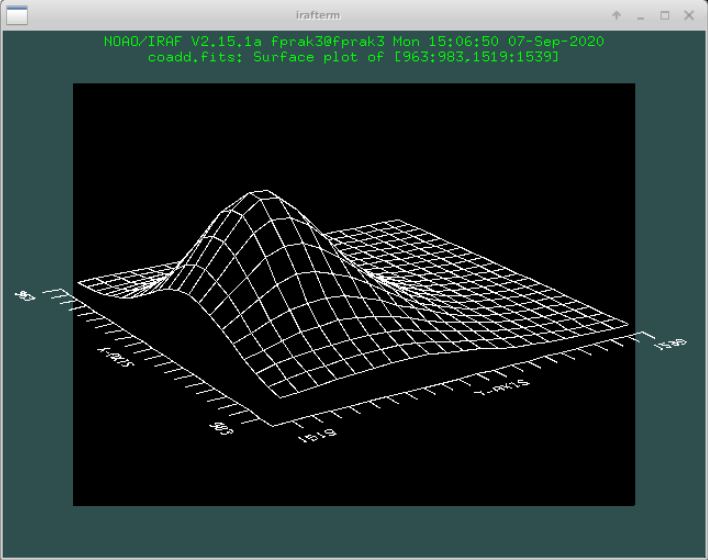
\includegraphics[width=0.9\linewidth]{starSurface.png}
   \end{center}
   \caption{Surface plot}
   \end{subfigure}
   \caption{Example plots of a star}%
   \label{fig:starPlots}
\end{figure}

Target contains two images, so its FWHM lies in between stars and galaxies at \num{8.71} pixels. Plots of target appear a bit different as well, see figure.~\ref{fig:targetPlots}. While surface plot do have some rough edges, column plot gives us the definite answer that this objects contains two images.
\begin{figure}[ht]
   \centering
   \begin{subfigure}[t]{0.5\textwidth}
   \begin{center}
   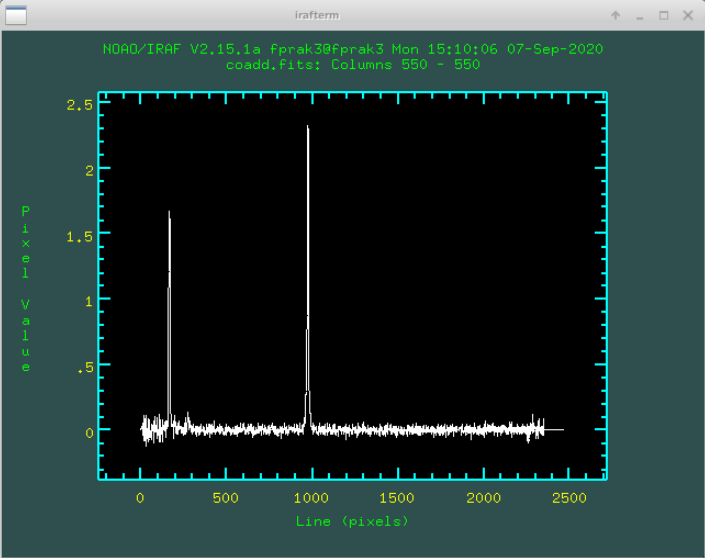
\includegraphics[width=0.9\linewidth]{targetColumn.png}
   \end{center}
   \caption{Column plot}
   \end{subfigure}%
   \begin{subfigure}[t]{0.5\textwidth}
   \begin{center}
   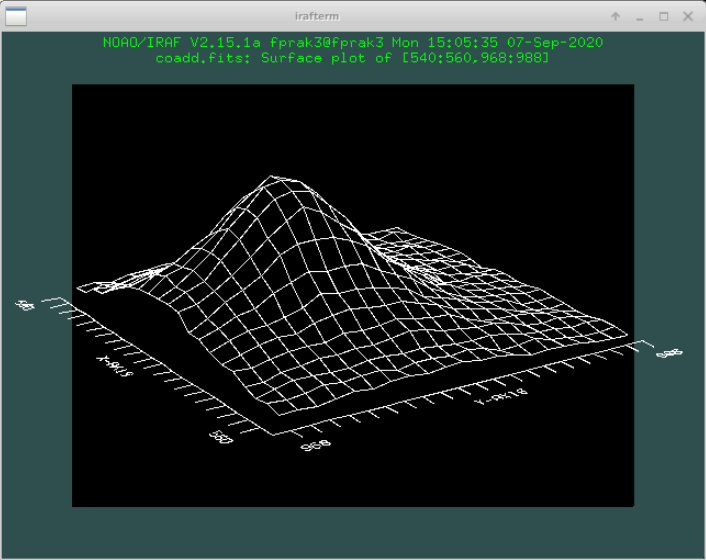
\includegraphics[width=0.9\linewidth]{targetSurface.png}
   \end{center}
   \caption{Surface plot}
   \end{subfigure}
   \caption{Example plots of the target}%
   \label{fig:targetPlots}
\end{figure}

Now to extract PSFs, a \verb|csh| shell script \verb|create_psf.csh| is used. The script takes four inputs: \verb|DIR| the directory containing the images, \verb|LIST| containing outputs of \verb|imexam| of selected stars and the target, \verb|Radius| size of square getting cut, and \verb|MAX_FWHM_STACK| the maximal size of PSF. One needs to use stars, since they are quasi-point-like sources. Stars brighter (higher flux) than the target need to be included in \verb|LIST|. \textcolor{blue}{Why?} \verb|RADIUS| is set to \num{30} pixels and \verb|MAX_FWHM_STACK| to \num{8.5}. \verb|LIST| file can be found in~\ref{app:LIST}.

Outputs of \verb|create_psf.csh| are each individual cut-outs \verb|cut_scale*.fits| and stacked PSF \verb|cut_star_stack_scale.fits|. Inspection of \verb|cut_star_stack_scale.fits| shows that there is no contribution from neighbouring stars, see figure~\ref{fig:stackSurface}. MFWHM of the stacked image is \num{8.09} as expected. Its surface plot is quite a smooth hump, even smoother than the hump of a single star. In the subsequent component fitting, the stacked image will be used, since all fluctuations/errors are averaged out.
\begin{figure}[ht]
	\begin{subfigure}[t]{0.5\textwidth}
	\begin{center}
		\includegraphics[width=0.95\linewidth]{screenshots-cut_star_stack_scale.fits.png}
	\end{center}
	\caption{The Stacked image in ds9}%
	\label{fig:stackScrenn}
	\end{subfigure}%
	\centering
	\begin{subfigure}[t]{0.5\textwidth}
	\begin{center}
	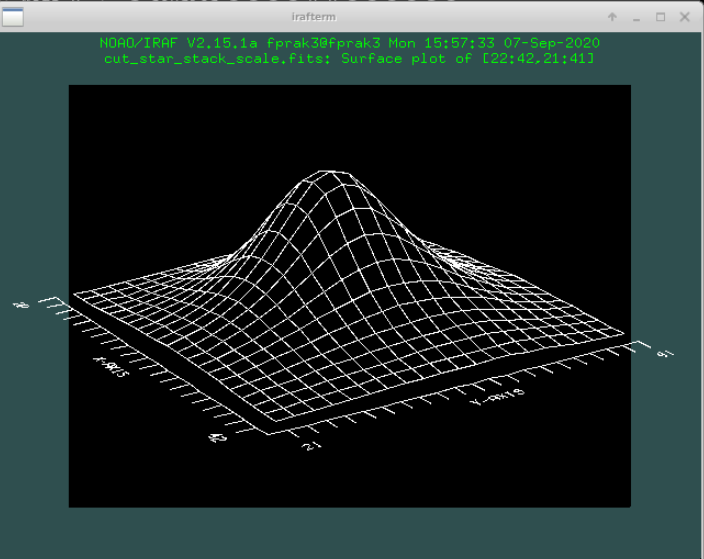
\includegraphics[width=0.9\linewidth]{stackSurface.png}
	\end{center}
	\caption{Surface plot of stacked image}%
	\label{fig:stackSurface}
	\end{subfigure}
\end{figure}

\clearpage
\section{Component fitting}
Although two images are blended, one can still try to use component fitting to find out individual flux and their separation. The 2d fitting program \verb|galfit| is used here.

\verb|galfit| is able to fit sky value in images and sky background is important to compute the $\sigma$-image~\cite{galfitManual}. Sky value is a fit parameter in \verb|galfit|, thus one need to compute it using \verb|imstats| and \verb|dfits| for normalisation: sky=\SI{1.71}{\per\s}. This value is then added into the image with \verb|ic| command provided in~\cite{manual}.

Input parameters of fitting are stored in \verb|galfit.input|, listed in appendix.~\ref{app:galfit}. Most important things are positions of two images, relative magnitude. These are just rough estimates as initial guess. Sky background is the third component of the fitting and sky ADU counts from previous part are given as input.

Execution of component fitting with the given parameter list outputs a log file \verb|fit.log| and a image block, see figure~\ref{fig:galfitOut}. The log file contains the coordinates of two images
\begin{equation*}
	(29.69, 24.71), (31.11, 31.16)
\end{equation*}
magnitude difference $1.70$, and $\chi^2/\nu = \num{44.542}$. From the residuals, one can see that the fitting works properly. They are quite uniformly distributed with some fluctuation, except there is a slightly bright spot at bottom. As suggested by the tutors, it could be caused by neighbouring stars. 
\begin{figure}[ht]
	\centering
	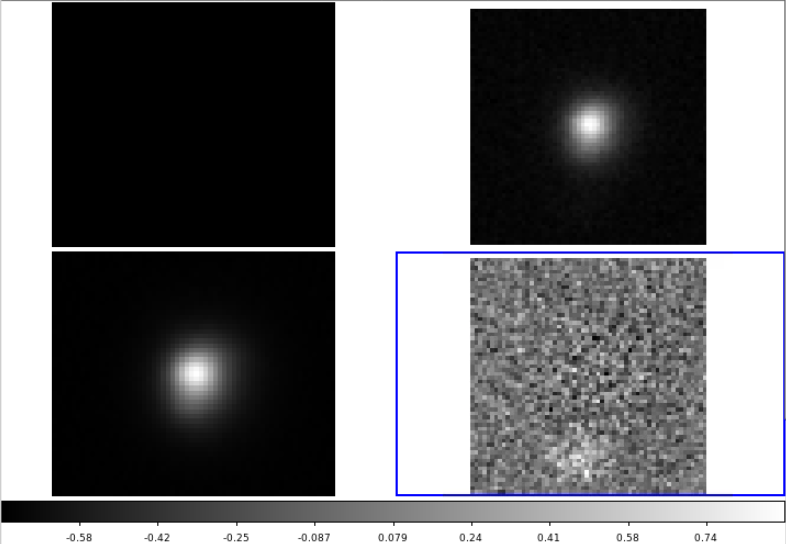
\includegraphics[width=0.8\linewidth]{galfitOutput.png}
	\caption{The image block generated by galfit assuming there are \textit{two} images. First image is intended to be empty. Second and third are respectively original and modelled images. Last one shows the residuals.}%
	\label{fig:galfitOut}
\end{figure}

One could also wonder if the target could consist only of one image, since it appears to be so visually. Another fitting is done but only with two components, one PSF fit and one sky background. Resultant image block is figure~\ref{fig:galfitOneOut}. There is a clear dark spot in the residual plot and $\chi^2/\nu = 101.615$, much worse than previous fitting. So the image cannot be explained by just one image.
\begin{figure}[ht]
	\centering
	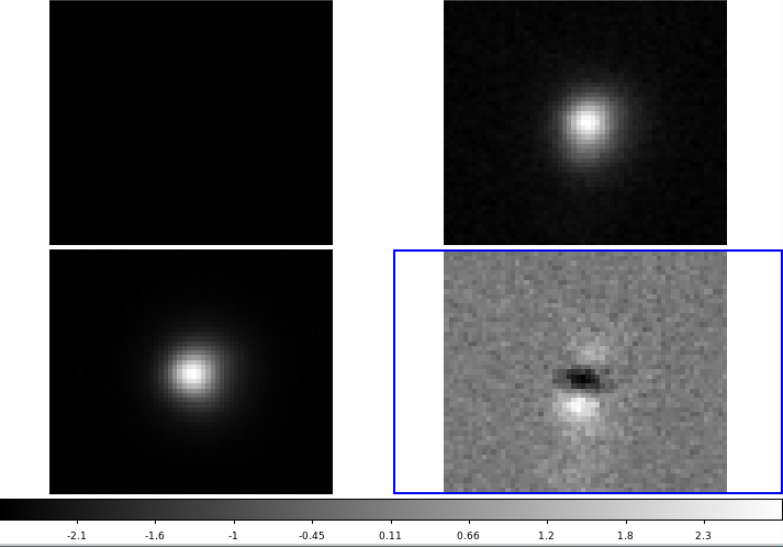
\includegraphics[width=0.8\linewidth]{galfitOneOutput.png}
	\caption{The image block generated by galfit assuming there is only \textit{one} image. First image is intended to be empty. Second and third are respectively original and modelled images. Last one shows the residuals.}%
	\label{fig:galfitOneOut}
\end{figure}

\clearpage
\section{Time-delay estimate} 
Time delay between two images can be estimated using minimal dispersion method. But a large number of observations are needed for it to work. Thus we take the data of~\cite{vuissoz} and the raw data are presented in appendix.~\ref{app:timdel}.

\begin{figure}[H]
	\centering
	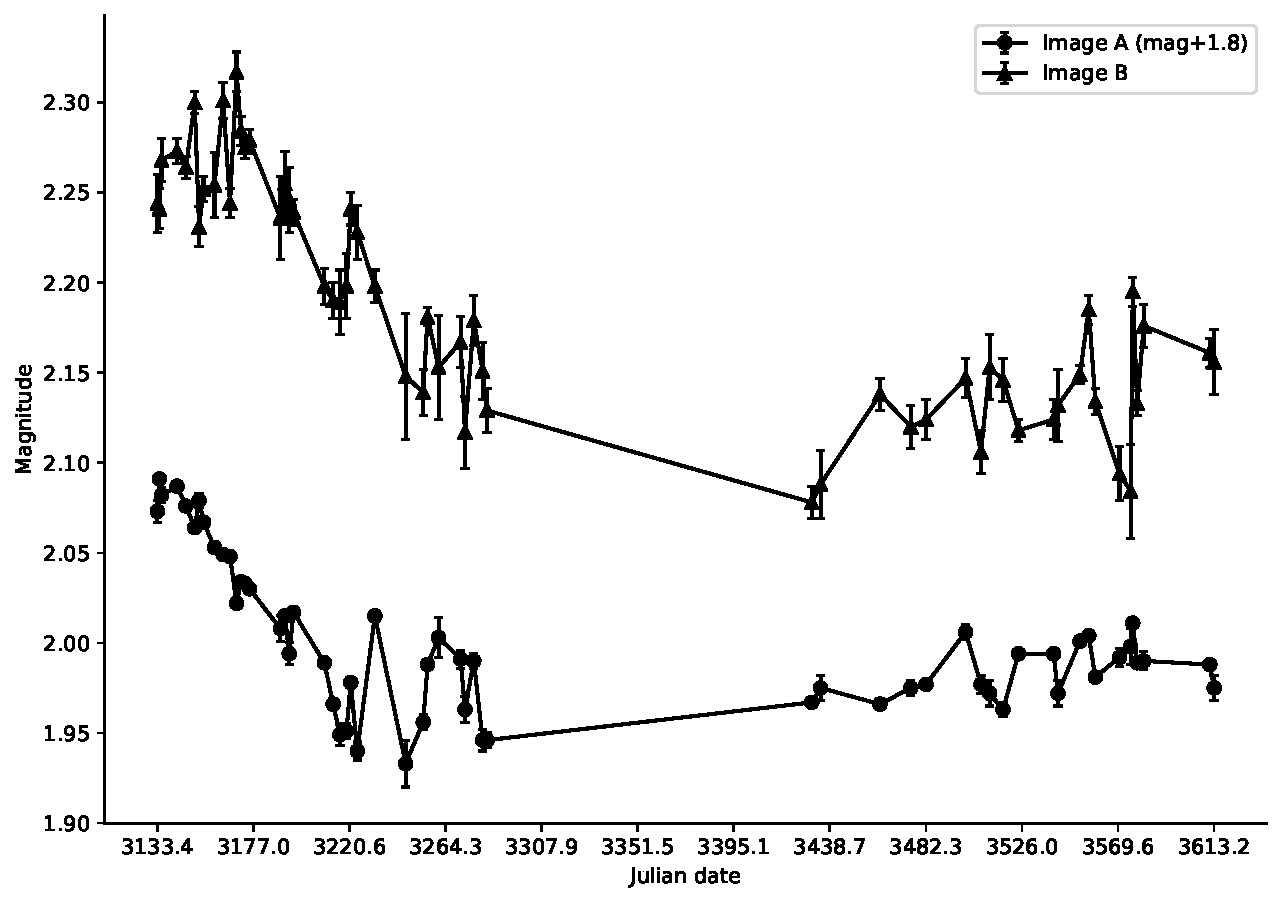
\includegraphics[width=0.7\linewidth]{timeDelay.pdf}
	\caption{Light curves of two images. Note that image A is originally much dimmer. For better comparison, its magnitude is added with $1.8$.}%
	\label{fig:timeDelay}
\end{figure}
Before using minimal dispersion method, one can try to inspect the light curves visually. Figure.~\ref{fig:timeDelay} shows the light curves. Most noticeable feature is a large gap between observations caused by rotation/spin of the Earth. Time delay is quite hard to discern in this plot, but if there is it should be $\order{10}$ days. There is also quite a magnitude difference.

To reliably determine time delay of two images, one has to use minimal dispersion method, implemented in program \verb|tdel|. Before using Monte Carlo, one should roughly find good input parameters of the program, so that the true global minimum can be found. Parameters are listed in table.~\ref{tab:tdelInParam}.

\begin{figure}[ht]
	\centering
	\begin{subfigure}[t]{\textwidth}
	\begin{center}
		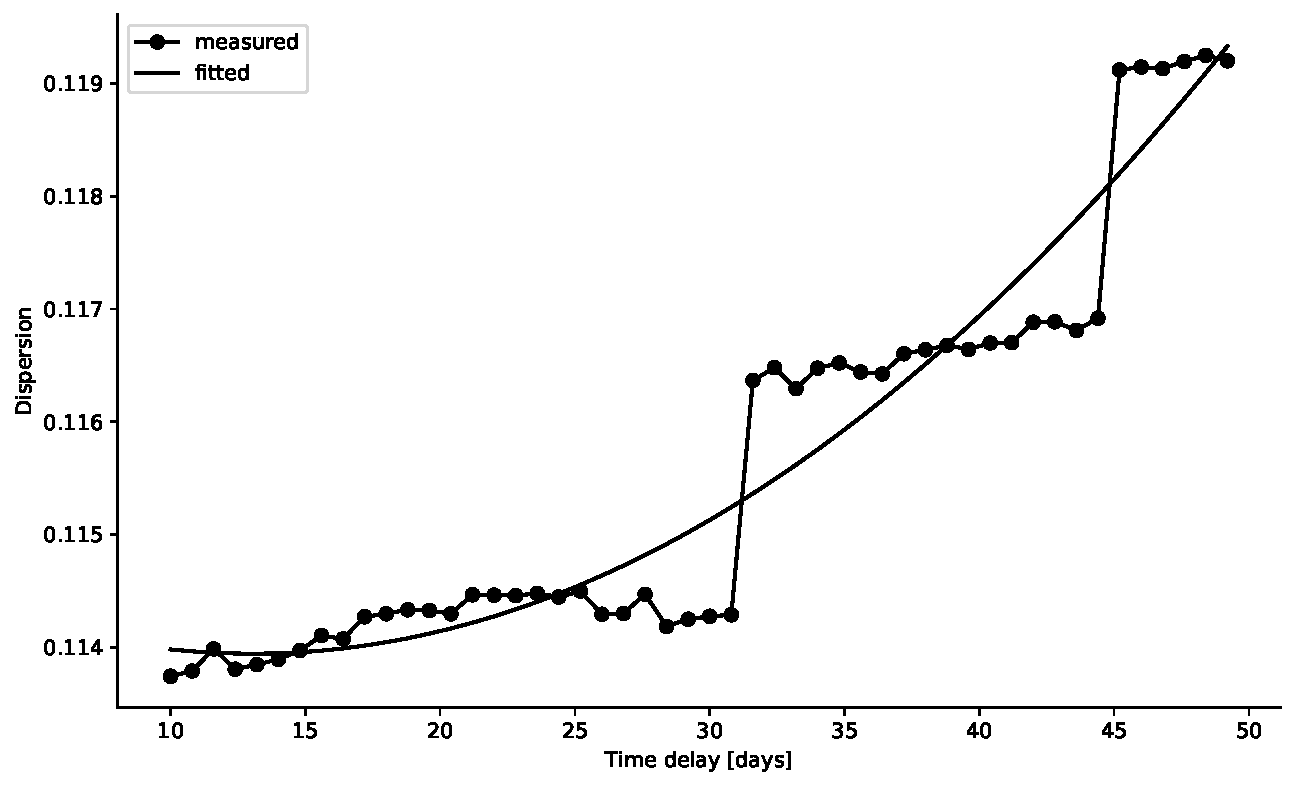
\includegraphics[width=0.6\linewidth]{disp.out_magshiftbin_0.dat.pdf}
	\end{center}%
	\caption{magnitude shift=\num{-2.5}}
	\label{fig:disp1}
	\end{subfigure}
	\begin{subfigure}[t]{\textwidth}
	\begin{center}
		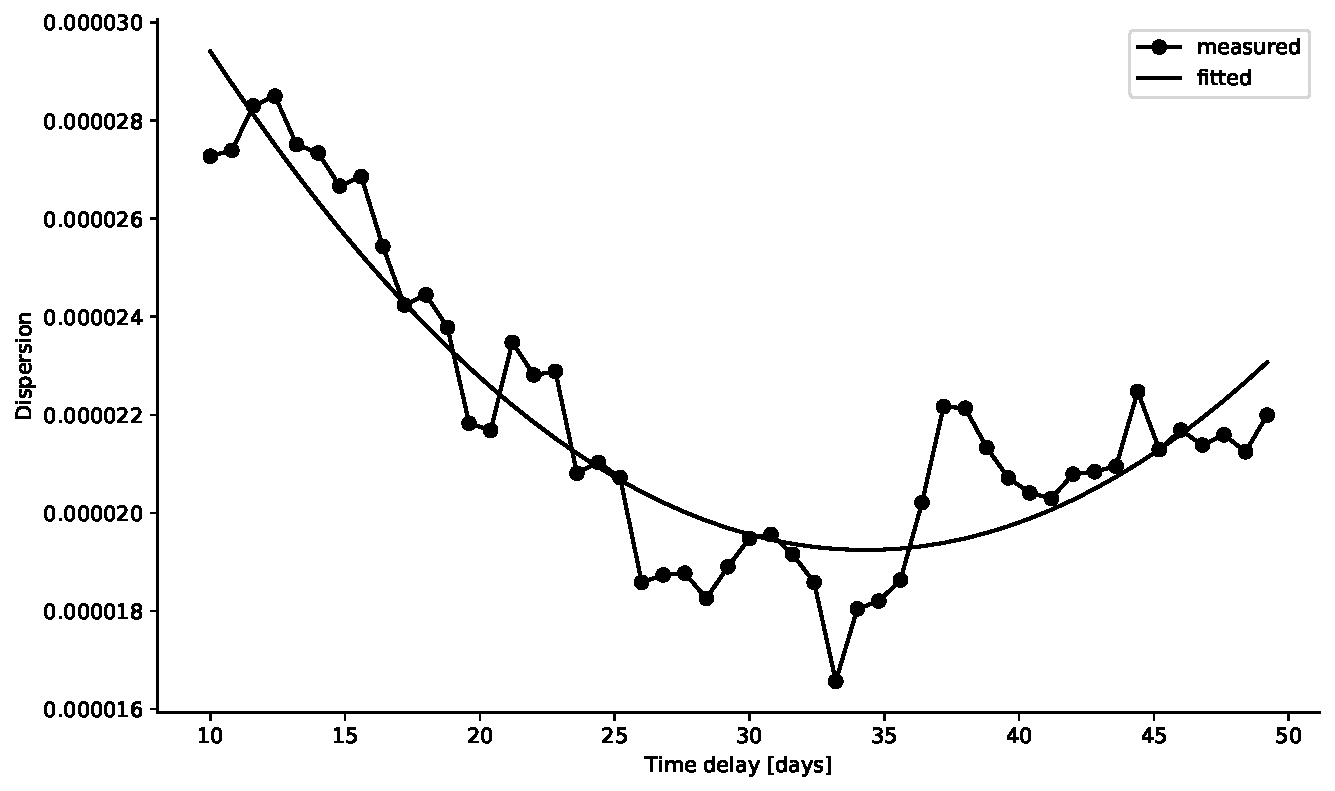
\includegraphics[width=0.6\linewidth]{disp.out_magshiftbin_25.dat.pdf}
	\end{center}%
	\caption{magnitude shift=\num{0}}
	\label{fig:disp2}
	\end{subfigure}
	\begin{subfigure}[t]{\textwidth}
	\begin{center}
		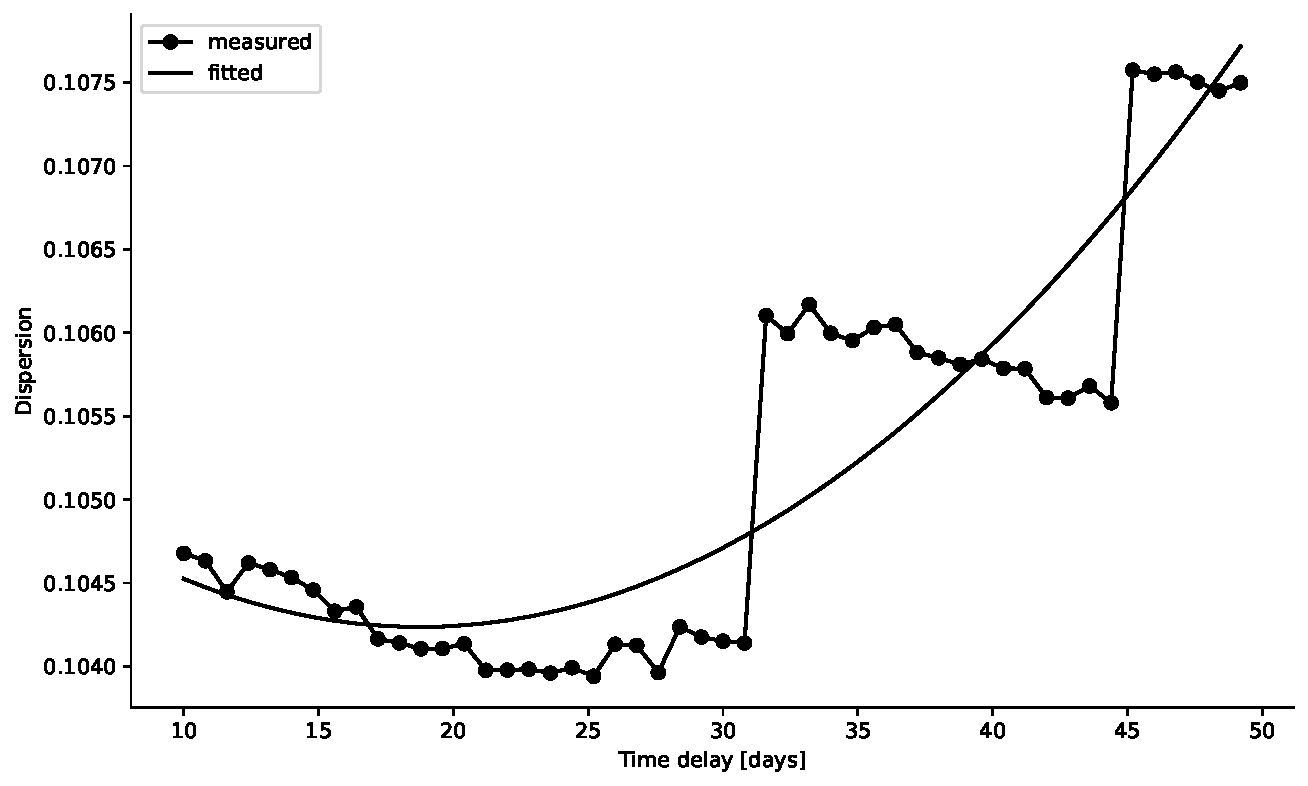
\includegraphics[width=0.6\linewidth]{disp.out_magshiftbin_49.dat.pdf}
	\end{center}%
	\caption{magnitude shift=\num{2.4}}
	\label{fig:disp3}
	\end{subfigure}%
	\caption{Dispersion spectra with various magnitude shifts.}%
	\label{fig:disp}
\end{figure}
Time delay is determined to be
\begin{equation}
	\lambda = \num{34.29}	
\end{equation}
Dispersion spectra of this preliminary run are figure.~\ref{fig:disp1},~\ref{fig:disp2}, and~\ref{fig:disp3}. Note the magnitude shift here refers to the magnitude shift after an initial adjustment, so that in the end minimal dispersion should be located at somewhere near zero magnitude shift. Indeed, the dispersion spectra show no clear minima within the selected region, except for zero magnitude shift. So we are certain that we found a global minimum.

With this knowledge and input parameters, Monte Carlo is turned on and it gives us
\begin{equation}
	\lambda = \num{34.336 +- 2.184}
\end{equation}

Here Monte Carlo method also gives us probabilities of various time delays, see figure.~\ref{fig:MCprob}. Fitting using function
\begin{equation*}
	f(t) = \frac{1}{\sigma \sqrt{2\pi}} \exp(-\frac{1}{2} \frac{(t-\mu)^2}{\sigma^2}) 
\end{equation*}
determined the parameters and covariance matrix to be
\begin{align*}
	\mu &= 33.959 \\
	\sigma &= 1.988 \\
	\Sigma &= \begin{pmatrix} 0.0064 & -0.0002 \\ -0.0002 & 0.004 \end{pmatrix}
\end{align*}
Note that here the fit function does not have either multiplicative or additive constant, since we have probability directly. These values are very close to direct output of Monte Carlo. So one may say the result of Monte Carlo is realistic.
\begin{figure}[ht]
	\centering
	\includegraphics[width=0.6\linewidth]{MCprob.pdf}
	\caption{Probability of different time delays estimated by Monte Carlo method. Raw data in appendix.~\ref{app:MCout}}%
	\label{fig:MCprob}
\end{figure}
\section{Lensing analysis}
